 %__       __ ________ ________ __    __  ______  _______   ______  __        ______   ______  __      __ 
%|  \     /  \        \        \  \  |  \/      \|       \ /      \|  \      /      \ /      \|  \    /  \
%| ▓▓\   /  ▓▓ ▓▓▓▓▓▓▓▓\▓▓▓▓▓▓▓▓ ▓▓  | ▓▓  ▓▓▓▓▓▓\ ▓▓▓▓▓▓▓\  ▓▓▓▓▓▓\ ▓▓     |  ▓▓▓▓▓▓\  ▓▓▓▓▓▓\\▓▓\  /  ▓▓
%| ▓▓▓\ /  ▓▓▓ ▓▓__      | ▓▓  | ▓▓__| ▓▓ ▓▓  | ▓▓ ▓▓  | ▓▓ ▓▓  | ▓▓ ▓▓     | ▓▓  | ▓▓ ▓▓ __\▓▓ \▓▓\/  ▓▓ 
%| ▓▓▓▓\  ▓▓▓▓ ▓▓  \     | ▓▓  | ▓▓    ▓▓ ▓▓  | ▓▓ ▓▓  | ▓▓ ▓▓  | ▓▓ ▓▓     | ▓▓  | ▓▓ ▓▓|    \  \▓▓  ▓▓  
%| ▓▓\▓▓ ▓▓ ▓▓ ▓▓▓▓▓     | ▓▓  | ▓▓▓▓▓▓▓▓ ▓▓  | ▓▓ ▓▓  | ▓▓ ▓▓  | ▓▓ ▓▓     | ▓▓  | ▓▓ ▓▓ \▓▓▓▓   \▓▓▓▓   
%| ▓▓ \▓▓▓| ▓▓ ▓▓_____   | ▓▓  | ▓▓  | ▓▓ ▓▓__/ ▓▓ ▓▓__/ ▓▓ ▓▓__/ ▓▓ ▓▓_____| ▓▓__/ ▓▓ ▓▓__| ▓▓   | ▓▓    
%| ▓▓  \▓ | ▓▓ ▓▓     \  | ▓▓  | ▓▓  | ▓▓\▓▓    ▓▓ ▓▓    ▓▓\▓▓    ▓▓ ▓▓     \\▓▓    ▓▓\▓▓    ▓▓   | ▓▓    
 %\▓▓      \▓▓\▓▓▓▓▓▓▓▓   \▓▓   \▓▓   \▓▓ \▓▓▓▓▓▓ \▓▓▓▓▓▓▓  \▓▓▓▓▓▓ \▓▓▓▓▓▓▓▓ \▓▓▓▓▓▓  \▓▓▓▓▓▓     \▓▓    
%.:..:..:..:..:..:..:..:..:..:..:..:..:..:..:..:..:..:..:..:.
\chapter{Methodology}
The project was to be executed in the following sequence:
\begin{enumerate}[label=\roman*.]
	\item Simulate IEEE 802.11 standard \gls{OFDM} on MATLAB over an \gls{AWGN} channel.
	\item Obtain average \gls{PAPR} performance of the simulated system.
	\item Simulate the \gls{OFDM} system over a Rayleigh fading channel.
	\item Simulate the \gls{OFDM} system over a Rician fading channel.
	\item Obtain \gls{BER} performance of all simulated systems.
	\item Use MATLAB's regression tools to derive an expression for the \gls{BER} curves generated.
\end{enumerate}

%,;,;,;,;,;,;,;,;,;,;,;,;,;,;,;,;,;,;,;,;
\section{OFDM Simulation}
The communication system was to be modeled in MATLAB. The blocks in the diagrams that follow would have analogous objects programmed to represent them.
\subsection{OFDM Transmitter}
The transmitter:
\begin{figure}[htpb!]
	\centerline{\resizebox{15cm}{!}{\input{Graphics/Methodology/OFDM_T_BLK.pdf_tex}}}
	\caption{OFDM Transmitter Block Diagram}
	\label{fig:ofdm_t_meth}
\end{figure}
\begin{figure}[htpb!]
	\centerline{\resizebox{!}{0.935\textheight}{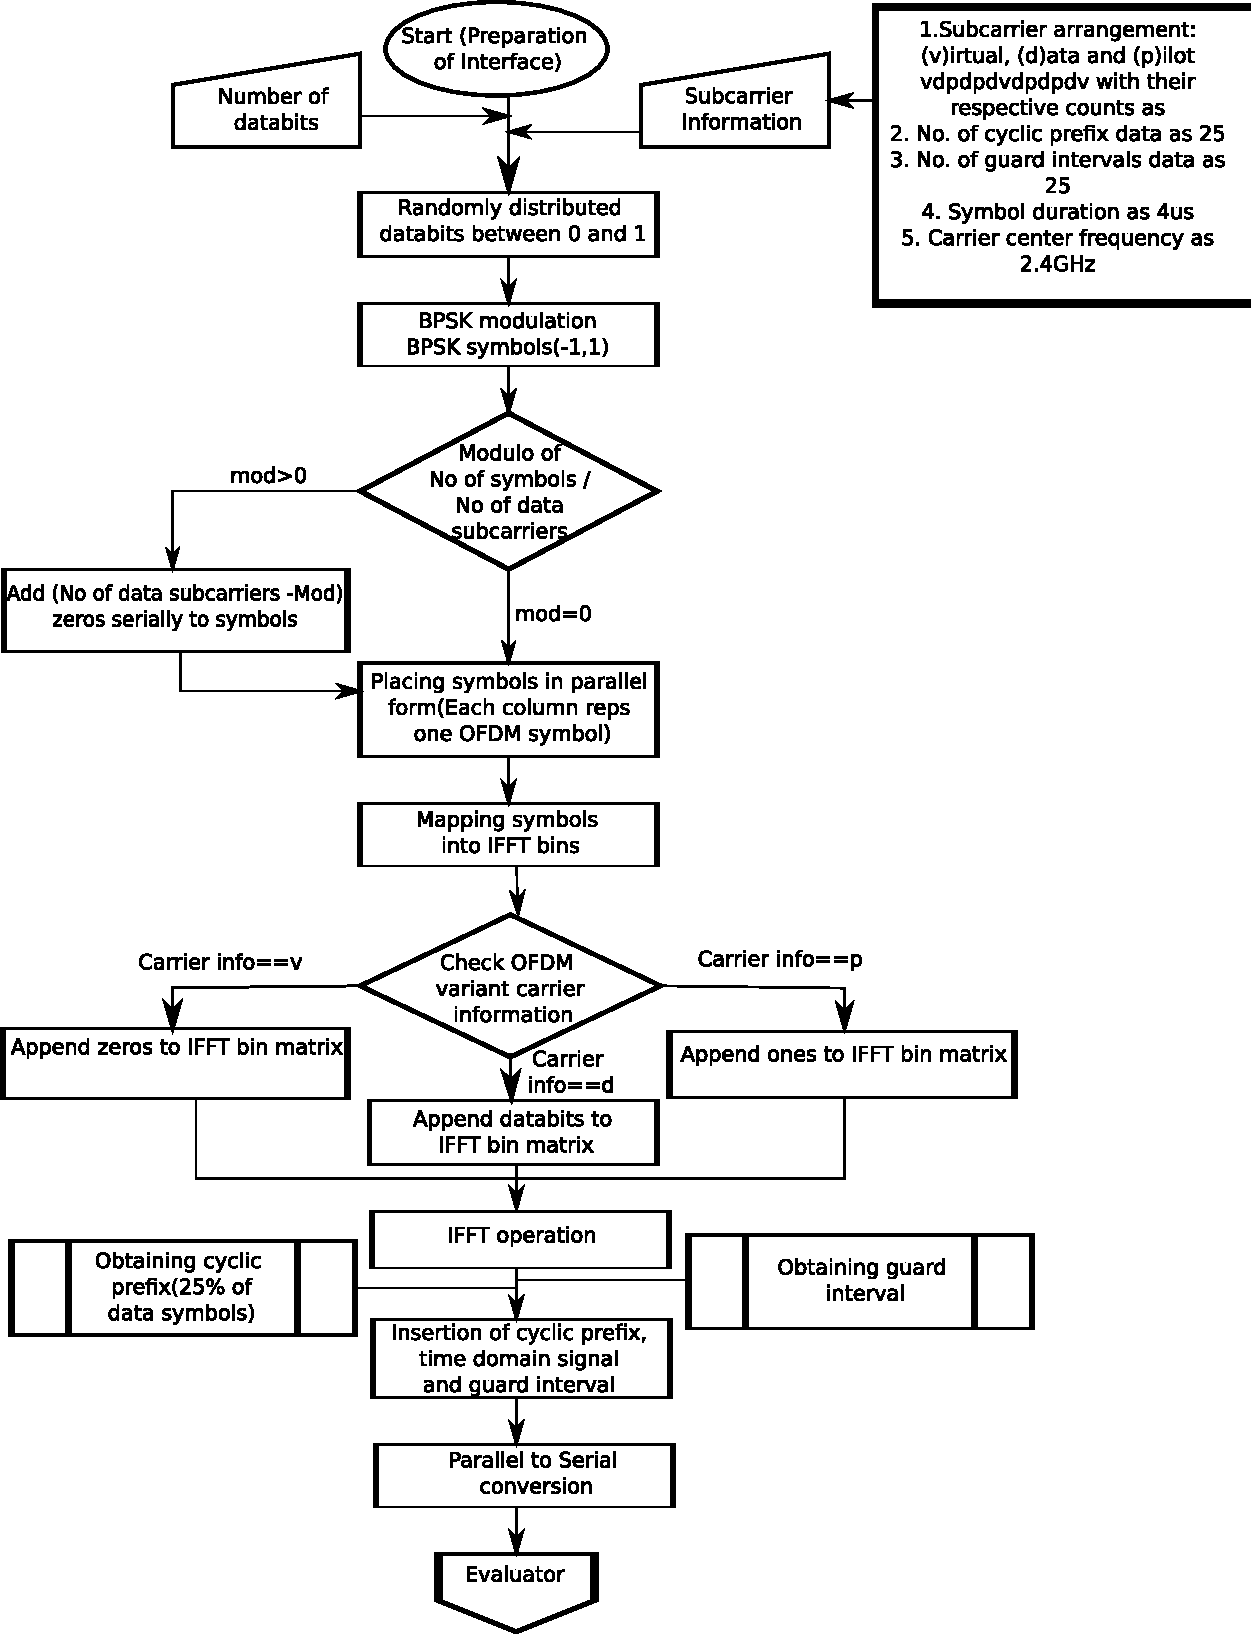
\includegraphics{Graphics/Methodology/Transmitter_flowchart.pdf}}}
	\caption{Transmitter Flowchart}
	\label{fig:system_transmitter}
\end{figure}

\pagebreak


\subsection{Channel}
The channel models that will be simulated are:
\subsubsection{AWGN Channel}
This channel adds white Gaussian noise to the signal as it is propagated through. 
\begin{figure}[htpb!]
	\centerline{\resizebox{15cm}{!}{\input{Graphics/Methodology/OFDM_CH_AWGN_BLK.pdf_tex}}}
	\caption{AWGN channel Block Diagram}
	\label{fig:ofdm_ch_awgn_meth}
\end{figure}

\subsubsection{Rayleigh Fading Channel}
The Rayleigh fading channel assumes no specular components in the transmitted signal. The signal Rayleigh fading has a Rayleigh Distribution.
\begin{figure}[htpb!]
	\centerline{\resizebox{15cm}{!}{\input{Graphics/Methodology/OFDM_CH_RAYL_BLK.pdf_tex}}}
	\caption{Rayleigh Fading Channel Block Diagram}
	\label{fig:ofdm_ch_rayl_meth}
\end{figure}

\subsubsection{Rician Fading Channel}
The Rician fading channel has multipath components as with the Rayleigh fading channel but has, in addition, a dominant line-of-sight component. The strength of the specular component determines the shape of the Rician distribution. 
\begin{figure}[h!]
	\centerline{\resizebox{15cm}{!}{\input{Graphics/Methodology/OFDM_CH_RICE_BLK.pdf_tex}}}
	\caption{Rician Fading Channel Block Diagram}
	\label{fig:ofdm_ch_rice_meth}
\end{figure}


\begin{figure}[htpb!]
	\centerline{\resizebox{!}{0.935\textheight}{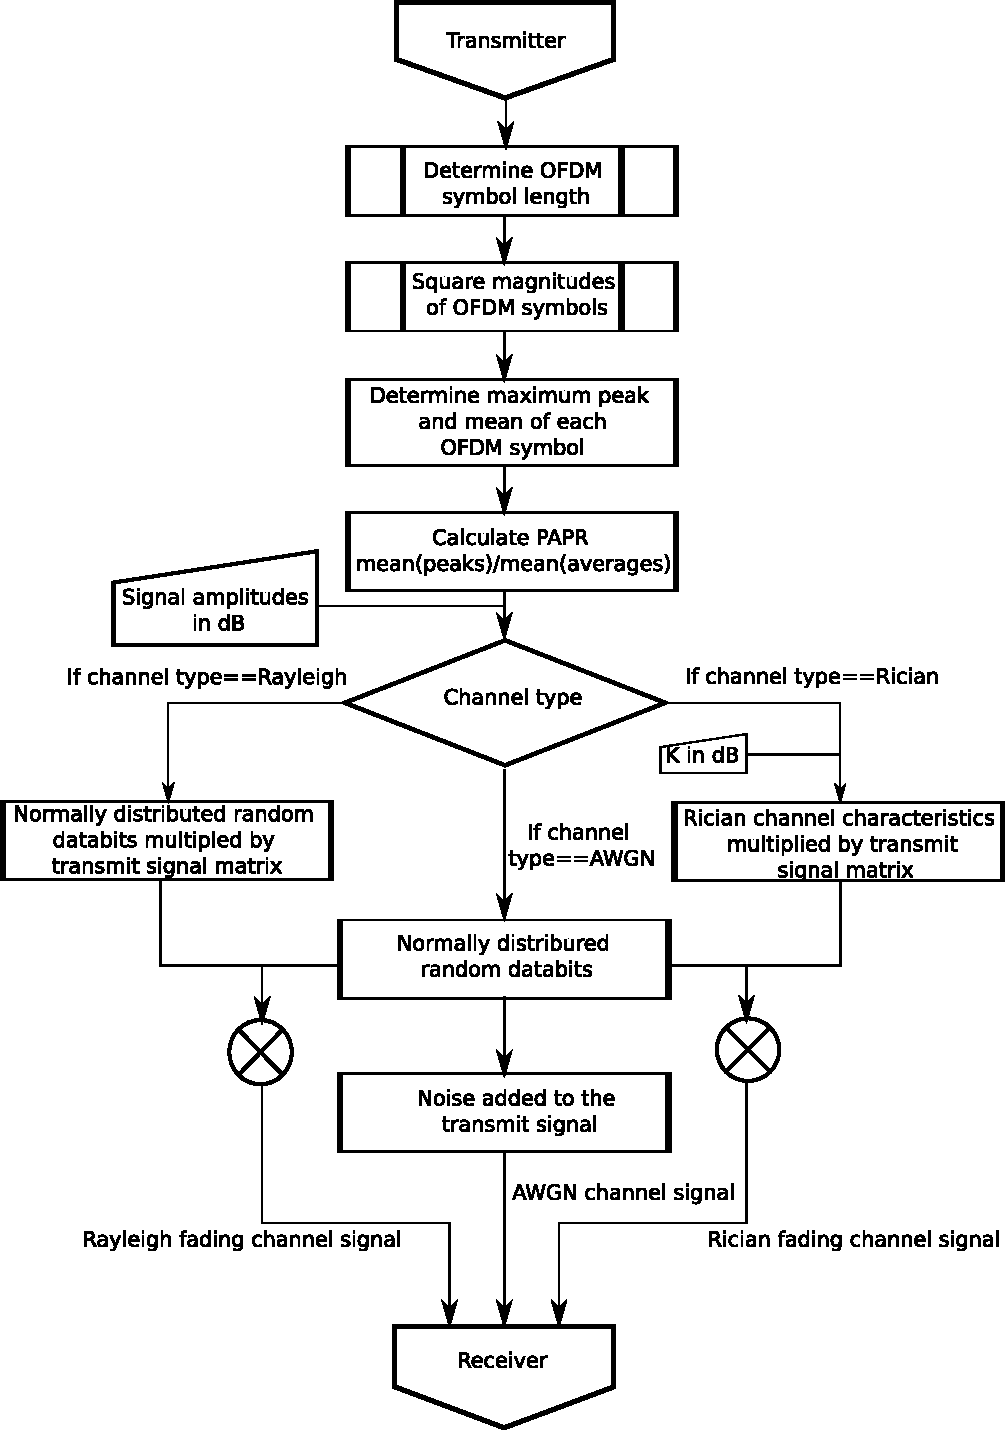
\includegraphics{Graphics/Methodology/Channel_flowchart.pdf}}}
	\caption{Channel Flowchart}
	\label{fig:ofdm_channel_meth}
\end{figure}
\pagebreak


\subsection{OFDM Receiver}
The receiver:
\begin{figure}[htpb!]
	\centerline{\resizebox{15cm}{!}{\input{Graphics/Methodology/OFDM_R_BLK.pdf_tex}}}
	\caption{Receiver Block Diagram}
	\label{fig:ofdm_r_meth}
\end{figure}
\begin{figure}[htpb!]
	\centerline{\resizebox{!}{0.935\textheight}{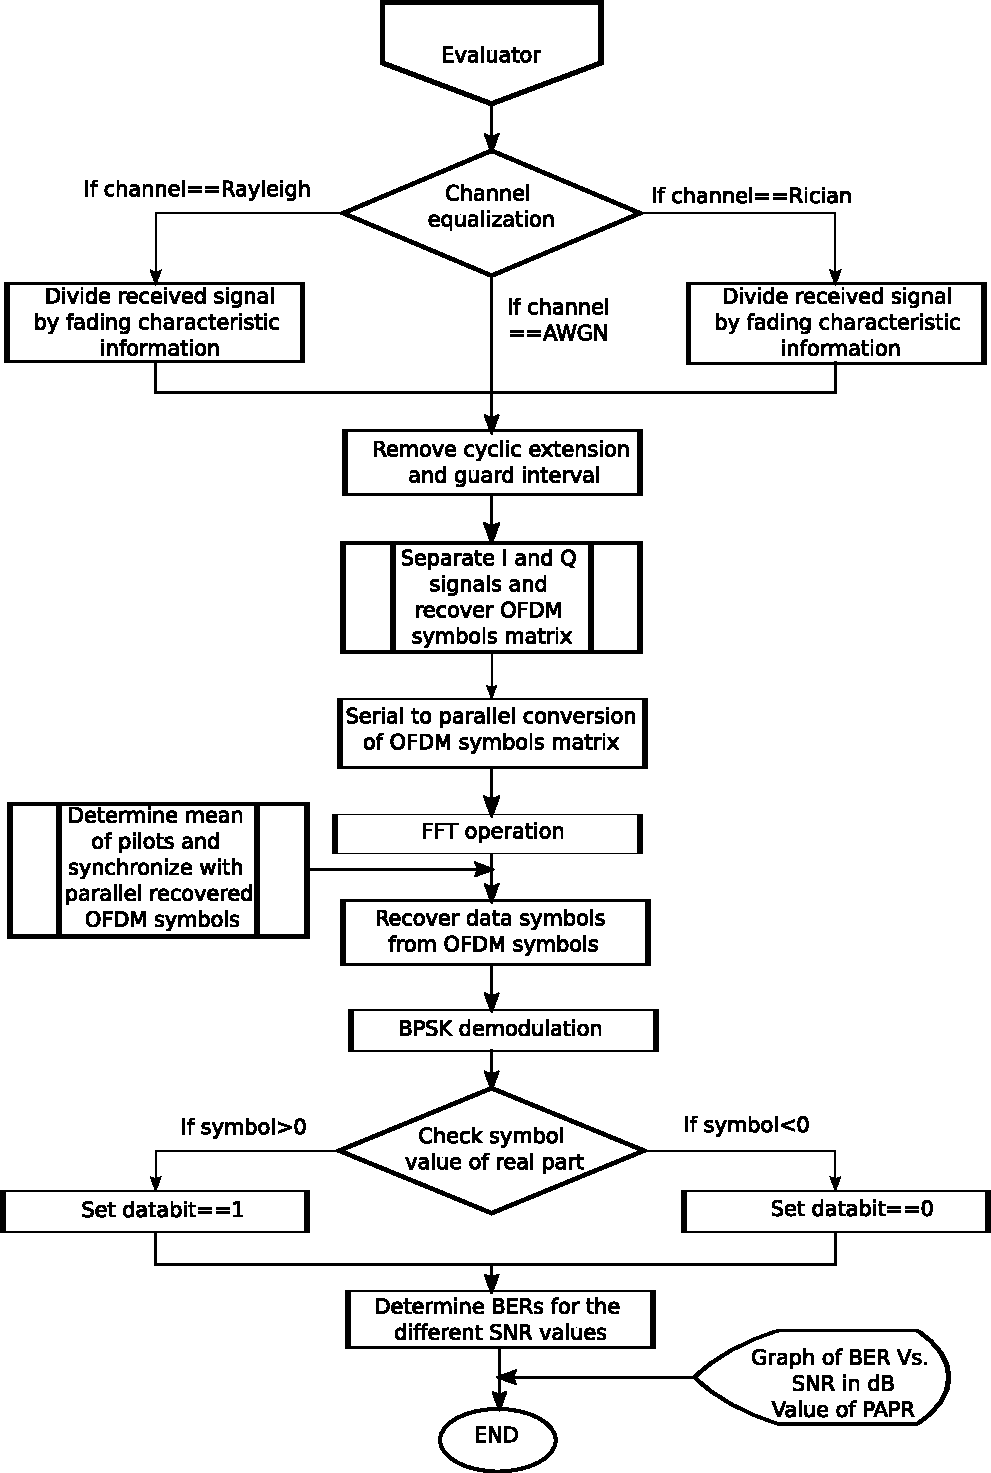
\includegraphics{Graphics/Methodology/Receiver_flowchart.pdf}}}
	\caption{Receiver Flowchart}
	\label{fig:ofdm_receiver_meth}
\end{figure}


\pagebreak

%,;,;,;,;,;,;,;,;,;,;,;,;,;,;,;,;,;,;,;,;
\subsection{BER Evaluation}
The system's \gls{BER} performance is to be evaluated within \gls{simulink} as well. The equivalent implementation would be as in figure \ref{fig:ber_blk_meth}
\begin{figure}[htpb!]
	\centerline{\resizebox{15cm}{!}{\input{Graphics/Methodology/BER_BLK.pdf_tex}}}
	\caption{\gls{BER} Evaluation}
	\label{fig:ber_blk_meth}
\end{figure}

%,;,;,;,;,;,;,;,;,;,;,;,;,;,;,;,;,;,;,;,;
\section{PAPR Evaluation}
\gls{PAPR} is evaluated at the transmitter output. To achieve this measurement, the peak amplitude is sampled over several symbol durations then its square divided by the square of the average signal amplitude.
\begin{figure}[!h]
	\centerline{\resizebox{10cm}{!}{\input{Graphics/Methodology/PAPR_BLK.pdf_tex}}}
	\caption{\gls{PAPR} Evaluation}
	\label{fig:papr_blk_meth}
\end{figure}
\pagebreak
%,;,;,;,;,;,;,;,;,;,;,;,;,;,;,;,;,;,;,;,;
\section{Curve fitting}

To determine the expressions for  the resulting BER curves from the system's simulation, \(Q\) function curves are fitted onto a line of best fit from the resulting BER data points:
%`;,`;,`;,`;,`;,`;,`;,`;,`;,`;,`;,`;,`;,`;,`;,`;,`;,`;,`;,`;,
\subsection{Rayleigh and Gaussian Models Curve Fitting}
From empirical observation over multiple simulation instances, see figure \ref{res:fig:Kvariation}, it was determined that the positions of the Gaussian and Rayleigh \gls{BER} curves are constant. To fit them to a curve, the \(Q\) function was scaled and shifted until it aligned perfectly with the curve. For higher \gls{SNR}s, a different Q function applied for both models.

%`;,`;,`;,`;,`;,`;,`;,`;,`;,`;,`;,`;,`;,`;,`;,`;,`;,`;,`;,`;,
\subsection{Rician Model Curve Fitting}
Obtaining a general expression for Rician fading followed these steps:
\begin{itemize}
	\item The system was simulated with Rician fading model over values of \(K\) ranging from 0 to 10 in increments of 1, as in figure \ref{res:fig:Kvariation}.
	\item For each curve, a scaled and shifted \(Q\) function was fitted. See figure \ref{fig:riceCurveFit}.
		\begin{equation}
			y(x) = aQ\left(\frac{x - b}{c}\right)
		\end{equation}
		\begin{mathDef}
			\mathSymb{a}{\(y\) axis scaling}
			\mathSymb{b}{\(x\) axis shift}
			\mathSymb{c}{\(x\) axis scaling}
		\end{mathDef}
	\item The values obtained are:
		\begin{center}
			\begin{tabular}{r r r r}
				\(K\)~dB & \(a\) & \(b\) & \(c\) \\
				\hline
				10 & 0.4 & 8.5 & 1.9 \\
				9 & 0.4 & 8.7 & 1.95 \\
				8 & 0.4 & 8.9 & 2 \\
				7 & 0.4 & 9.1 & 2.1 \\
				6 & 0.41 & 9.4 & 2.2 \\
				5 & 0.41 & 9.8 & 2.35 \\
				4 & 0.41 & 10.1 & 2.53 \\
				3 & 0.42 & 10.5 & 2.55 \\
				2 & 0.425 & 10.8 & 2.6 \\
				1 & 0.43 & 11 & 2.69 \\
				0 & 0.44 & 11.1 & 2.72
			\end{tabular}
		\end{center}
	\item These values are then plotted as in figure \ref{fig:findKcoeff} and fitted to a curve which relates their value to \(K\). This yields the expressions:
		\begin{align}
			a &= \begin{cases}0.0004K^2 - 0.0081K + 0.4392 & 0 \leq K < 5\\0.4 & 5 \leq K\end{cases}\label{eq:meth:a}\\
			b &= -0.2855K + 11.522\label{eq:meth:b}\\
			c &= -0.0917K + 2.785 \label{eq:meth:c}
		\end{align}
\end{itemize}
\begin{figure}
	\centering
	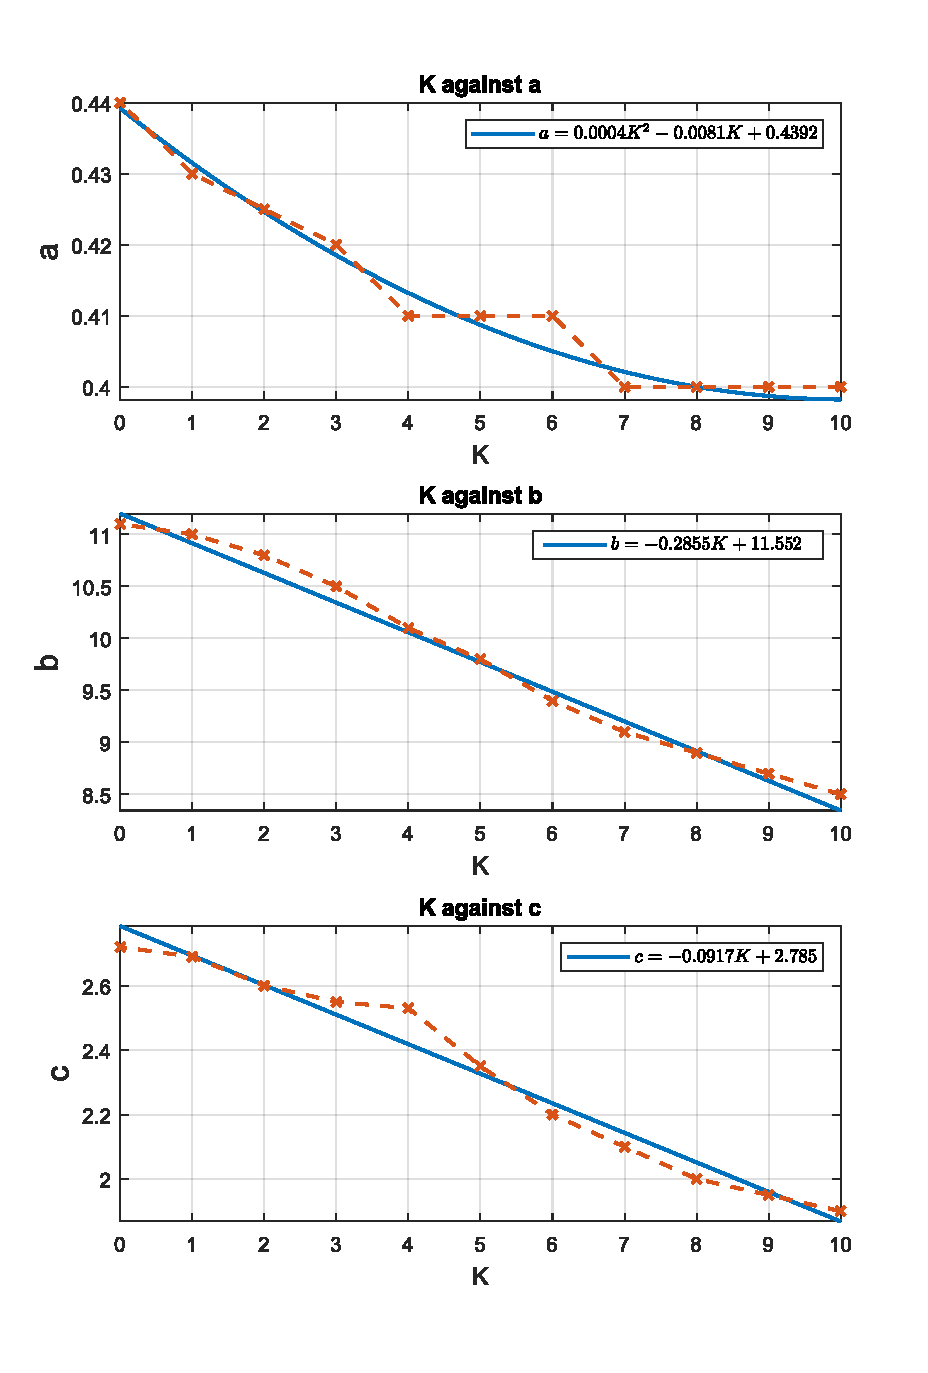
\includegraphics[width=\textwidth]{Graphics/Methodology/KcoeffFit.pdf}
	\caption{Relation of \(a\), \(b\) and \(c\) to \(K\)}
	\label{fig:findKcoeff}
\end{figure}
